\section{Node Fingerprint} \label{PingLoad}
In this section, we propose an attack named ``PingLoad''\footnote{Stands for `PINGing payLoad''.} which allows an adversary to actively fingerprint applications running on different nodes, and later use this information to identify an application running on a specific node.

\subsection{The PingLoad Attack}

In \Cref{Sec:DistinguishDevice}  we mentioned the fact that processor occupied by other tasks may prolong the PRI.  \Cref{PingloadExample} illustrates such an example.

\AddFigure{fig/PINGLOAD_Session.png}{PRI prolonged by Sensor Reading}{PingloadExample}

\Cref{PingloadExample} illustrates an example where the PING Request is received when the node is processing a sensor reading. In this example, the measured PRI would include part of  sensor reading plus the actual time required for processing the PING request.

The PingLoad attack exploits the facts that:
\begin{itemize}
	%Routine application
	\item Typically nodes in WSN applications perform routine operations, e.g. collect the temperature  information for every 10 seconds, etc. 
	%Low performance
	\item The performance of the devices are low such that the difference in PRIs can be observed in the network traffic. As a counter example, the differences in PRIs on a desktop machine would be too small to be observed.
	%Different PRIs
	\item PRI prolongs differently when the processor is occupied by different tasks.
\end{itemize}

%How the attack works.
Therefore when sending a large amount of PING packets to different node running different applications, those prolonged PRIs would show distinctive distributions for different nodes performing different operations. \Cref{PingLoadTheory} illustrates an example that reading temperature sensor and ALS prolongs PRIs differently. 

\begin{figure}[ht!]
	\center
	\begin{subfigure}{0.8\textwidth}
	{
		\center
		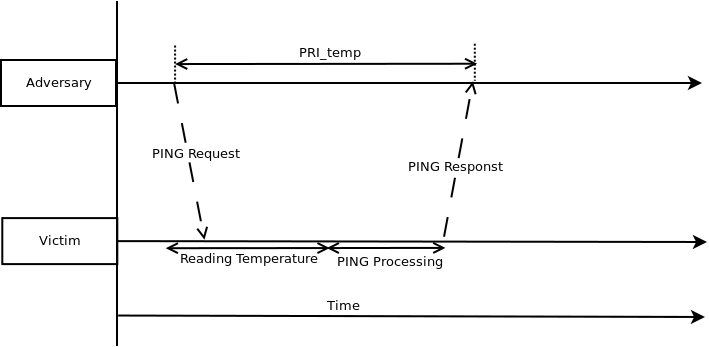
\includegraphics[width=\textwidth]{fig/PingLoad_temperature.png}
	}
	\subcaption{PRI when reading temperature sensor}
	\end{subfigure}
	\begin{subfigure}{0.8\textwidth}
	{
		\center
		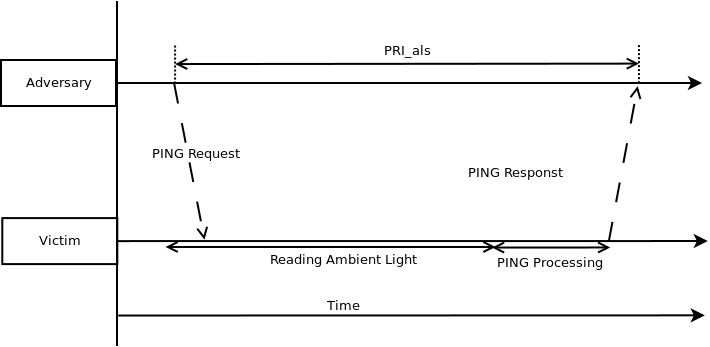
\includegraphics[width=\textwidth]{fig/PingLoad_als.png}
		\subcaption{PRI when reading Ambient Light Sensor(ALS)}
	}
	\end{subfigure}
	\caption{An example of reading temperature and ALS sensor results into different PRI.}
	\label{PingLoadTheory}
\end{figure}

The PingLoad attack hence uses such prolonged PRI distributions as fingerprints to different applications, matching an unknown application to known applications by finding  the statistically most similar PRI distribution. To be more specifically, the attack is described using a ``closed world'' setting with the following steps:

\begin{description}
	\item[Profiling]
	The first step requires the adversary to have the pre-knowledge of a set of applications, denote as $\mathbb{A} = \{A_1, A_2, ..., A_n\}$. The application to be identified, denote as $A_x$, is included in the set, i.e. $A_x \in \mathbb{A}$ where $x$ is known to the adversary.
	
	To fingerprint the applications, the adversary collects PRIs for each application in $\mathbb{A}$. We denote the profiled traces as:
\begin{equation}
\mathbb{T}_p = \{T_1, T_2, ..., T_n\}
\end{equation}
where $T_i$ is collected by repetitively sending PING request to a node running application $A_i$. Each trace $T_i$ contains multiple PRIs, denote as $T_i = \{PRI^i_1, PRI^i_2, ..., PRI^i_{m_i}\}$.

	\item[Collecting Trace]
	
	
	\item[Matching Fingerprint]

\end{description}

\subsection{Experiment}